
\section{Markov Decision Process}
	\subsection{Introduction to MDP}
	Recall that a Markvo Decision Process (MDP) is characterized by its fully observable environment. That being said, any RL problems can be transformed into MDP. \\
	The Markov Decision Process inherits from Markov Reward Process (MRP), which extends from the Markov Process (Markov Chain). 
	\paragraph{Definition} Markov Process (MP) is the tuple $ \langle \mathcal{S, P} \rangle $ where 
	\begin{itemize}
	\item $\mathcal{S}$ is the finite set of states
	\item $\mathcal{P}$ is the state transitional probability matrix. where an entry $\mathcal{P}^a_{ss'}$ is defined
	\begin{equation*}
	\mathcal{P}_{ss'} := \mathbb{P}[S_{t+1} = s' | S_t = s] 
	\end{equation*}
	\end{itemize}

	\paragraph{Definition} Markov Reward Process (MRP) is the tuple $ \langle \mathcal{S, P, R, \gamma} \rangle$ where 
	\begin{itemize}
	\item $\mathcal{R}$ is the reward function 
	\begin{equation*}
	\mathcal{R}_s = \mathbb{E}[R_t | S_t = s]
	\end{equation*}
	\item $\gamma$ is the discount factor, $\gamma \in [0,1]$
	\end{itemize}

	\paragraph{Definition} The return $G_t$ (not to be confused with reward $R_t$) is the total discounted reward from step t
	\begin{equation*}
	G_t = R_t + \gamma R_{t+1} + \gamma^2 R_{t+2} + ... = \sum^\infty_{i=0} \gamma^i R_{t+i}
	\end{equation*}

	\paragraph{Definition} The state value function $v(s)$ of an MRP gives the expected return.
	\begin{align*}
	v(s) &= \mathbb{E}[G_t | S_t = s] \\
	&= \mathbb{E}[R_{t+1} + \gamma R_{t+2} + \gamma^2 R_{t+3} + ... | S_t = s] \\
	&= \mathbb{E}[R_{t+1} + \gamma v(S_{t+1}) | S_t = s] \\
	&= \mathcal{R}_s + \gamma\sum_{s' \in \mathcal{S}}\mathcal{P}_{ss'}v(s')
	\end{align*}

	Notice the equation for the value function casted in matrix form is known as \textbf{Bellman Equation}. Concretely,
	\begin{align*}
	v &= \mathcal{R + \gamma P}v \\
	(\mathrm{I}- \gamma\mathcal{P})v &= \mathcal{R} \\
	v &= (\mathrm{I}- \gamma\mathcal{P})^{-1}\mathcal{R}
	\end{align*} 
	\begin{figure}[h]
	\centering
	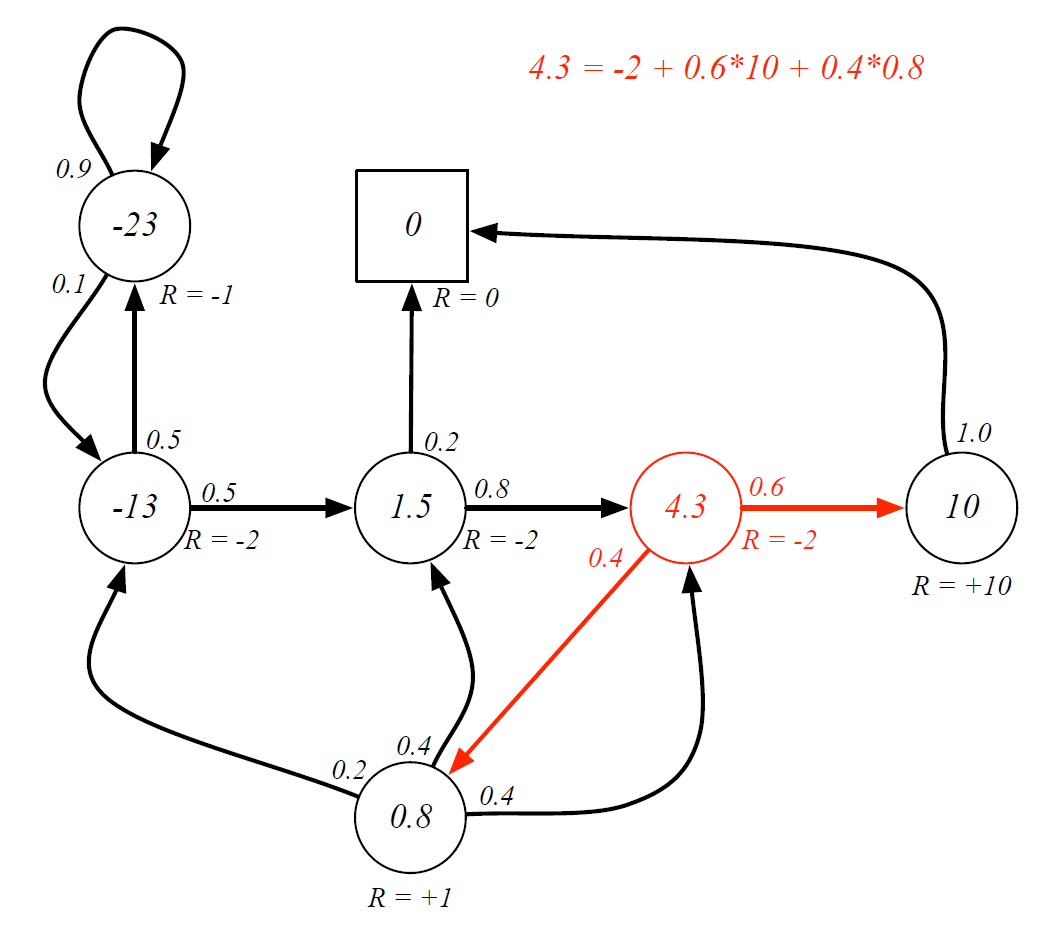
\includegraphics[scale=0.5]{ch2fig1.png}
	\caption{Value function of a Markov Reward Process}
	\end{figure}

	
	\subsection{Markov Decision Process}
	Finally, let's dig into the topic of today - the Markov Decision Process (MDP). MDP is an MRP with decisions, and states are Markov.
	\paragraph{Definition} The Markov Decision Process (MDP) is the tuple $\langle \mathcal{S, P, R, \gamma, A} \rangle$ where 
	\begin{itemize}
	\item $\mathcal{S}$ is the finite set of states
	\item $\mathcal{A}$ is the set of finite actions 
	\item $\mathcal{P}$ is the state transitional probability matrix. where an entry $\mathcal{P}^a_{ss'}$ is defined
	\begin{equation*}
	\mathcal{P}^a_{ss'} := \mathbb{P}[S_{t+1} = s' | S_t = s, A_t = a] 
	\end{equation*}
	\item $\mathcal{R}$ is the reward function 
	\begin{equation*}
	\mathcal{R}^a_s = \mathbb{E}[R_t | S_t = s, A_t = a]
	\end{equation*}
	\item $\gamma$ is the discount factor, $\gamma \in [0,1]$
	\end{itemize}

	\begin{figure}[h]
	\centering
	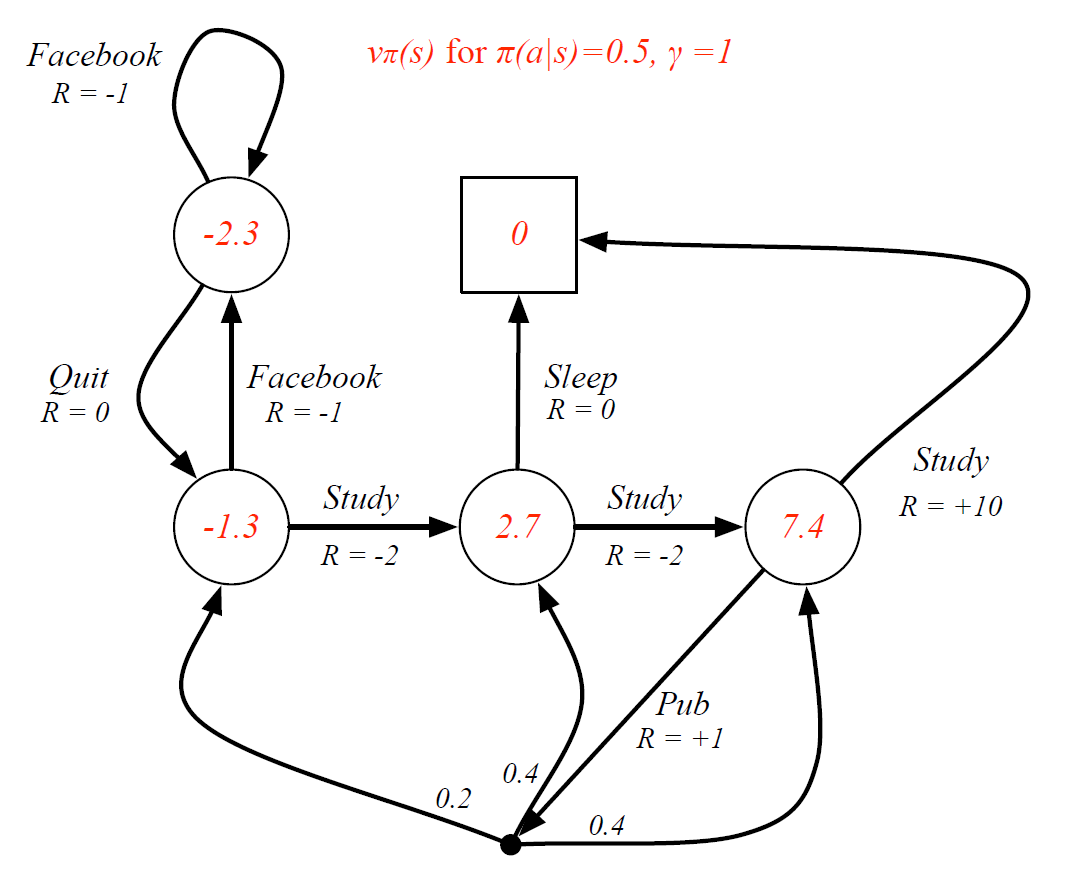
\includegraphics[scale=0.5]{ch2fig2.png}
	\caption{A Markov Decision Process}
	\end{figure}

	\paragraph{Definition} A policy (probabilistic) given by
	\begin{equation*}
	\pi(\mathbf{a|s}) = \mathbb{P}[A_t|S_t] 
	\end{equation*}
	defines the behavior of the agent, is stationary and dependent of the \underline{current state} (not history). 

	Note that the MDP $\langle \mathcal{S, P, R, \gamma, A} \rangle$ can be reduced to the MRP $ \langle \mathcal{S, P, R, \gamma} \rangle$ where
	\begin{itemize}
	\centering
	\item $\mathcal{P}^{\pi}_{ss'} = \sum_{a \in \mathcal{A}} \pi(\mathbf(a|s))\mathcal{P}^a_{ss'}$
	\item $\mathcal{R}^{\pi}_s = \sum_{a \in \mathcal{A}} \pi(\mathbf(a|s))\mathcal{R}^a_{ss'}$
	\end{itemize}


	\paragraph{Definition} The \textit{state-value} function is the expected return from state s following policy $\pi$
	\begin{equation*}
	v_\pi(s) = \mathbb{E}[G_t|S_t = s]
	\end{equation*}

	\paragraph{Definition} The \textit{action-value} function is the expected return from state s, \underline{taking action a}, and following policy $\pi$
	\begin{equation*}
	q_\pi(s,a) = \mathbb{E}[G_t|S_t = s, A_t = a]
	\end{equation*}

	The inter-dependent relationship of The action-value and state-value functions are captured by the following equation.
	\begin{align*}
	v_\pi(s) &= \sum_{a \in \mathcal{A}}  \pi(\mathbf{a|s)}q_\pi(s,a) \\
	q_\pi(s,a) &= \mathcal{R}^a_s + \gamma \sum_{s' \in \mathcal{S}} P^a_{ss'}v(s') 
	\end{align*}

	\begin{figure}[h]
	\centering
	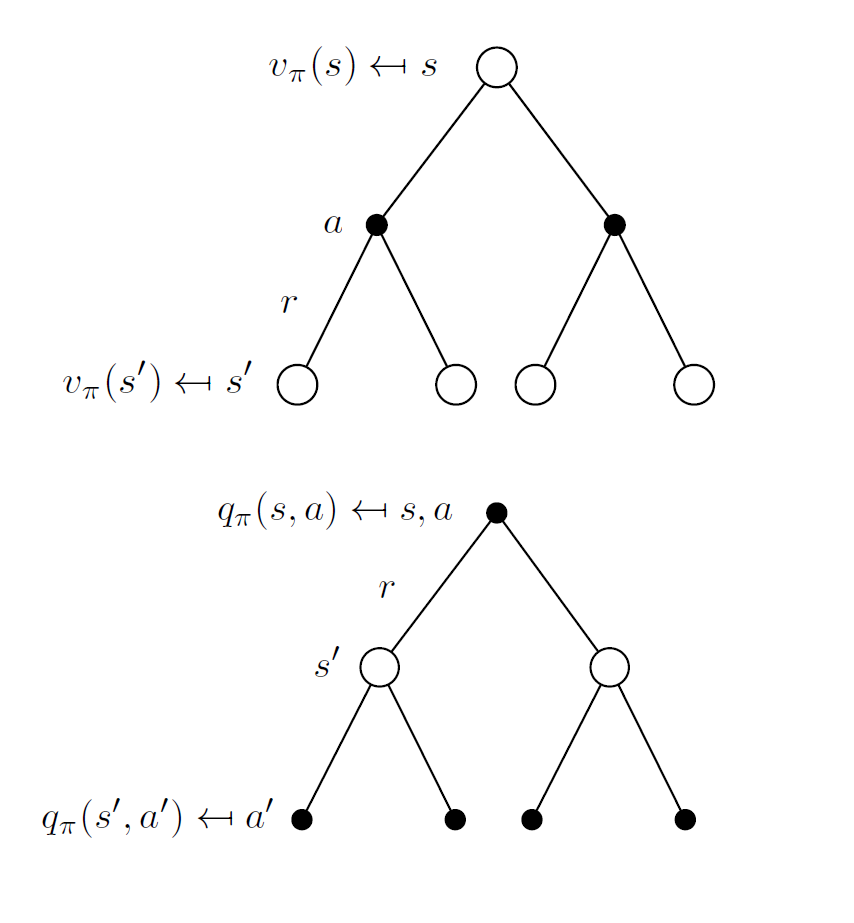
\includegraphics[scale=0.5]{ch2fig3.png}
	\caption{Recursive relation of value functions}
	\end{figure}

	Expressing the equations above in a recursive manner, we have the \textbf{Bellman Expectation Equation} 
	\begin{align*}
	v_\pi(s) &= \sum_{a \in \mathcal{A}}  \pi(\mathbf{a|s)} (\mathcal{R}^a_s + \gamma \sum_{s' \in \mathcal{S}} P^a_{ss'}v(s'))\\
	q_\pi(s,a) &= \mathcal{R}^a_s + \gamma \sum_{s' \in \mathcal{S}} P^a_{ss'}(\sum_{a' \in \mathcal{A}}  \pi(\mathbf{a'|s')}q_\pi(s',a')) 
	\end{align*}

	\begin{figure}[h]
	\centering
	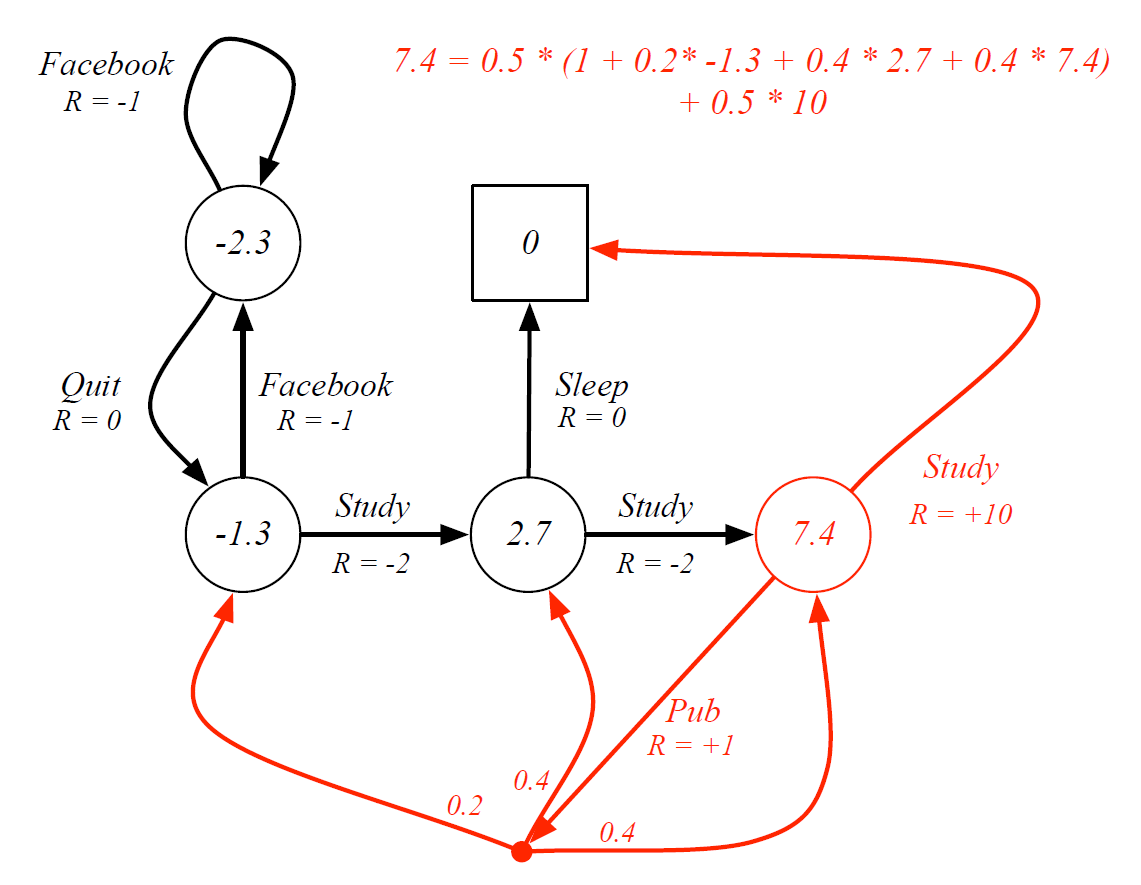
\includegraphics[scale=0.5]{ch2fig4.png}
	\caption{Computing state-value function using the Bellman Expectation Equation}
	\end{figure}

	\paragraph{Definition} The \textbf{ state-value function} $v_*(s)$ is said to be \textbf{optimal} if 
	\begin{equation*}
	v_*(s) = \max_\pi v_\pi (s)
	\end{equation*}
	Similarly, The \textbf{ action-value function} $q_*(s,a)$ is said to be \textbf{optimal} if 
	\begin{equation*}
	q_*(s,a) = \max_\pi q_\pi (s,a)
	\end{equation*}


	\begin{figure}[h]
	\centering
	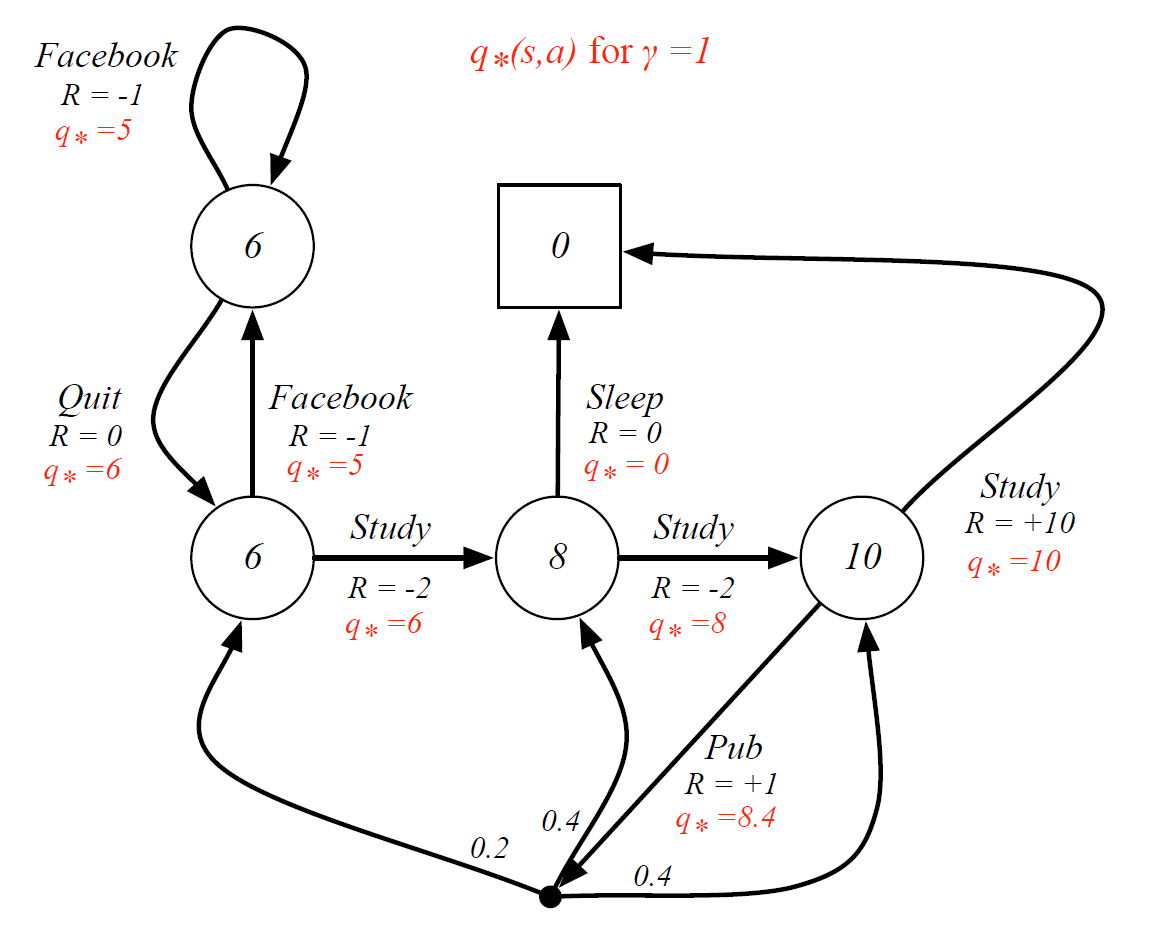
\includegraphics[scale=0.5]{ch2fig5.png}
	\caption{Computing optimal action-value function using the Bellman Optimality Equation}
	\end{figure}

	\paragraph*{Theorem}
	Define $\pi \ge \pi'$ iff $v_\pi(s) \ge v_{\pi}|(s)$, for any Markov Process,
	\begin{itemize}
	\item $\exists \, \pi_*$ such that $\pi_* \ge \pi$
	\item All optimal policies achieve the same optimal value function $v_{\pi_*}(s) = v_*(s)$
	\item All optimal policies achieve the same optimal action-value function $q_{\pi_*}(s,a) = q_*(s,a)$
	\end{itemize}

	\paragraph{Theorem}
	An optimal policy can be found by maximizing over $q_*(s,a)$ 
	\begin{equation*}
	\pi_*(\mathbf{a|s}) = \begin{cases}
	1, if a = \mathrm{argmax}_{a \in A} q_*(s,a)\\
	0, otherwise
	\end{cases}
	\end{equation*}

	\begin{figure}[h]
	\centering
	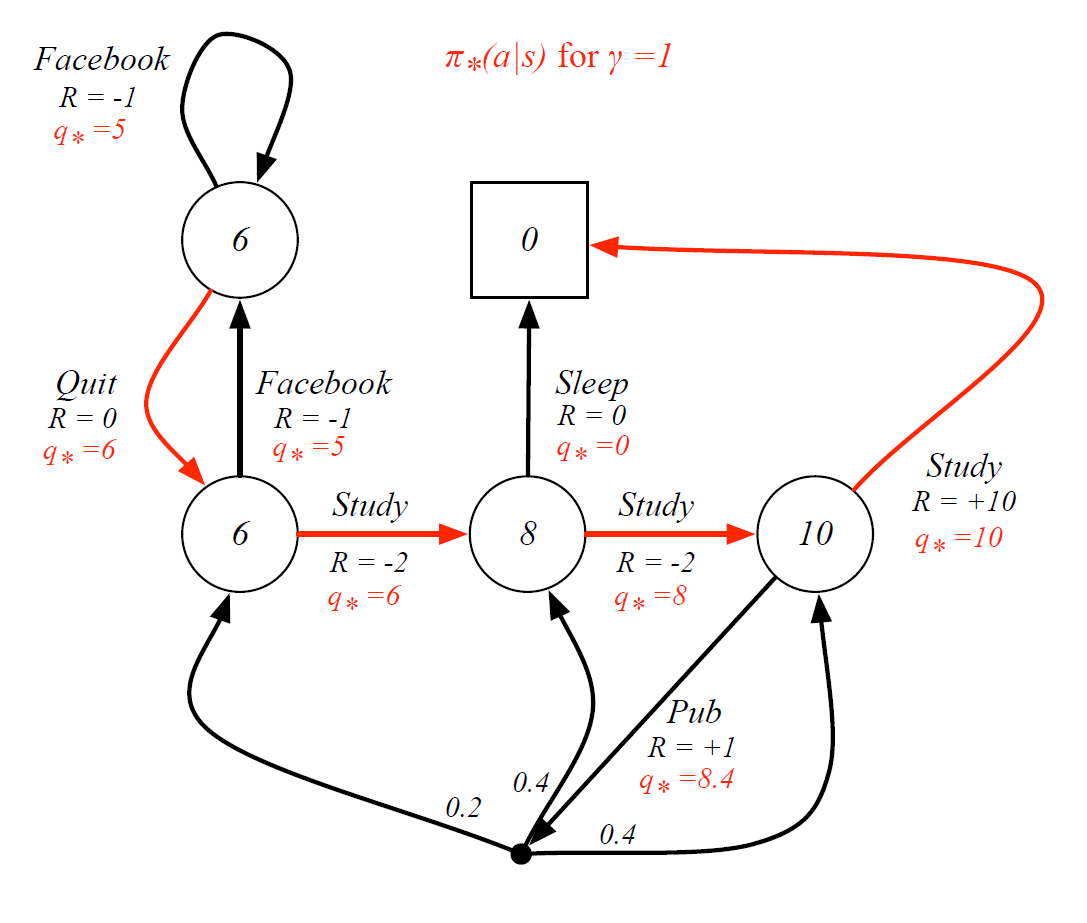
\includegraphics[scale=0.5]{ch2fig6.png}
	\caption{Finding the Optimal Policy}
	\end{figure}

	Finally, we summarize this chapter by introducing the \textbf{Bellman optimality Equation}
	\paragraph{Definition} The recursive definition of the optimal value function is given as the following:
	\begin{equation*}
	v_*(s) = \max_a q_*(s,a) = \max_a (\mathcal{R}^a_s + \gamma \sum_{s' \in \mathcal{S}}\mathcal{P}^a_{ss'}v_*(s'))
	\end{equation*}
	\begin{equation*}
	q_*(s,a) = \mathcal{R}^a_s + \gamma \sum_{s' \in \mathcal{S}} \mathcal{P}^a_{ss'} \max_{a'} q_*(s',a')
	\end{equation*}

	\begin{figure}[h]
	\centering
	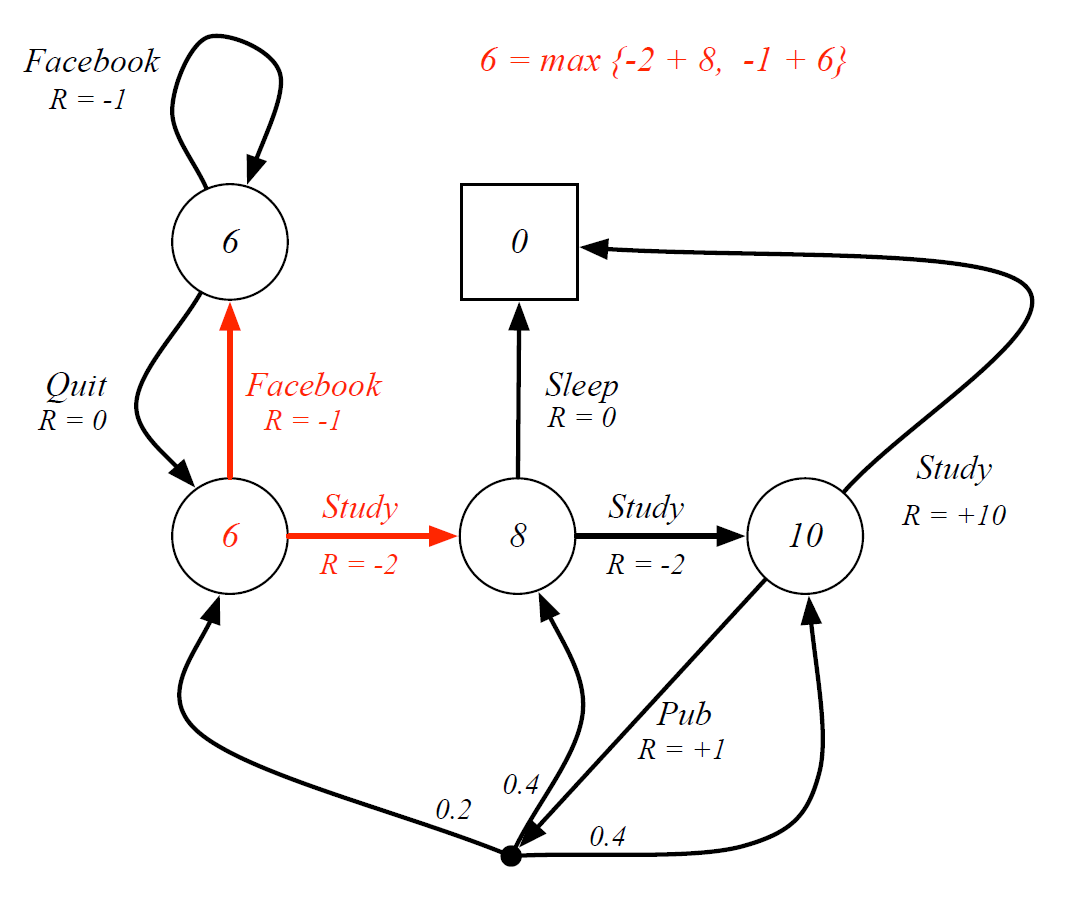
\includegraphics[scale=0.5]{ch2fig7.png}
	\caption{Finding Optimal value function $v_*(s)$}
	\end{figure}

	\subsection{Infinite MDPs}

	The 3 cases of infinite MDPS are listed as follows.
	\begin{enumerate}
	\item Countable infinite
	\end{enumerate}
	% \begin{align*}
	% \mathbf{y} &= \mathbf{Ax} \\
	% \begin{bmatrix} 3 \\ 3  \end{bmatrix} &= \begin{bmatrix} 1 & 1 \\ 1 & 1 \end{bmatrix} \begin{bmatrix} 2 & 2\\ 2 & 2 \end{bmatrix}
	% \end{align*}

	